		\documentclass{report}
		
		% Info
		\title{Cinematic storytelling in VR}
		\author{Wouter Vanmulken}
		\date{December 2017}
		
		% Packages 
		\usepackage{graphicx}
		\usepackage{hyperref}
		
		%Titles
		\usepackage[T1]{fontenc}
		\usepackage{titlesec, blindtext, color}

		\definecolor{gray75}{gray}{0.75}
		\newcommand{\hsp}{\hspace{20pt}}
		\titleformat{\chapter}[hang]{\Huge\bfseries}{\thechapter\hsp\textcolor{gray75}{|}\hsp}{0pt}{\Huge\bfseries}
		\setlength{\parindent}{0em}
		\setlength{\parskip}{1em}
		\usepackage[a4paper, total={6in, 8in}]{geometry}
		\usepackage[scaled]{helvet}
		\renewcommand\familydefault{\sfdefault} 
		\usepackage[T1]{fontenc}
		
		\usepackage{todonotes}
		\usepackage{gensymb}
		\usepackage{graphicx}
		\usepackage{float}
		
		\usepackage{cite}
%		\usepackage{apacite}
		
		\begin{document}
				\pagenumbering{gobble}
				\maketitle
				\tableofcontents
				\newpage
				\pagenumbering{arabic}
		
				\chapter{Introduction}
				
				This is a research paper about storytelling in VR. As there is still a lot of information undiscovered about storytelling in VR, i will also be talking about my personal observations on VR storytelling experiences. Therefore this document will mostly contain opinions on the current state and possibilities and should not be used as empirical evidence.\todo{maybe not rek your crdibility immediately}
				
				\chapter{Research questions}
		
				To be able to research the subject of Cinematic storytelling in VR, i made three questions to guide me through the process.
				\begin{itemize}
					\item How can we make people feel present in a story?
					\item How can we keep people from missing key story details?
					\item How can we grab the attention of a user?
				\end{itemize}

				My first intention of this research was to find how cinematic composition translates in VR. But composition in VR has a lot more aspects than just how a single image looks like. A VR storytelling experience is more like a play than a movie. And therefore i will look into how to get the users attention ,keeping it and if we even want to focus it.
				
				\todo{Couple the two pieces into eachother}

				
				\chapter{How can we make people feel present in a story ?}
				
				\section{Resources}		\todo{make a better title}		
				Making people feel present is a delicate balance, a world that doesn't feel right can be a big problem in a storytelling experience. A real-world example of this would be, someone talking during a movie. This often brings people back to reality and can be quite frustrating. Although this might be annoying when watching a movie, it can be quite devastating while in VR. Breaking the illusion of a virtual world even once can make it feel unreal or even more important, uninteresting.

				Currently there isn't a lot of official research on what these things might be in relation to cinematic experiences. But luckily there still is Oculus storytellingstudio. Storytellingstudio was a department of Oculus specifically set up to test how cinematic experiences in VR can be created. To research the subject they took the first steps into animating storytelling experiences. With the motto of "story is king", they are currently still \textbf{the} resource on storytelling in VR. 
				
				Unfortunately the department has been closed since they didn't want to compete in a marketplace they were creating research for. But not before they put a lot of the research online on their blog and making some amazing proof-of-concept pieces like Henry and Dear Angelica. Currently they are still the most valuable resources about storytelling in VR.
				
				The only way to really solve these problem is to make experiences. So i'm glad that there are companies like \href{http://www.penrosestudios.com/}{Penrose studios}, \href{http://www.baobabstudios.com/}{Baobab studios} and \href{https://with.in/}{Within} to take over the torch.

				%https://www.oculus.com/story-studio/blog/5-lessons-learned-while-making-lost/
				\section{Routine}
				
				When you go to a movie you start by buying a ticket then you maybe go buy some popcorn or some other snack. And after that you usually still have another 5 minutes of sitting there or some commercials. You mentally prepare yourself during this time and get in a different mindspace. This can be quite crucial in VR. Since we don't have a ticketbooth or popcorn stand. You're just instantly dropped into a new environment. 
				
				This often leads to people feeling overwhelmed and stop paying attention. There is so much to see that your story might not be that interesting compared to the environment. Therefore we need to give the users some time before actually starting the story. In this time they can acclimate to the environment and look around at the interesting world you created.
				
				To make such a routine you could use three phases.
				
				\subsection{Introduction}
				In this phase there shouldn't be much in the users environment. In Lost they storytelling studio used a black room with "fi the firefly". This phase is mostly designed for users who haven't had a lot of VR experience and are often overwhelmed the first time they are. So there is a dark room where a firefly flies and react around you. This way there is an introduction
				
				\todo{this}
				being in the envuronment but nothing happens
				
				actual story
				

				\todo{fi the firefly}
				
				\section{Common issues}
				\begin{itemize}
					\item Not being acknowledge in the world or the .
					\item Only one thing happening at a time in the world.
					\item Walking into objects.
				\end{itemize}
				
				
				\chapter{How can we keep people from miss key story details ?}
				
				You probably noticed that the title of the chapter is missing an "ing". This is just an example of how a users would feel, missing a part of the story in VR. Missing information can get quite frustrating as you can imagine, in this instance you probably blamed me and you would be right to do so. In a VR experience the same thing would happen. The user thinks your experience is poorly made and start to doubt the experience as well as feel stupid that they didn't notice the information.
				
				\todo{write the chapter}
				
				\chapter{How can we grab the attention of a user ?}
				
				\begin{figure}[h!]
					\centering
					
\includegraphics[width=\linewidth/3]{img/pow.jpg}
					\caption{Attention grabbing example.}
					\label{fig:pow}
				\end{figure}
				
				\section{Should we be guiding the users focus}
				Before we can even answer the question of how we can grab the attention we need to answer the question of if we should. VR gives us 360$^{\circ}$ vision of a alternate reality, so should we limit ourselves because we aren't used to it yet. When the first movie was projected, which was of a train coming into the station, people wanted to jump out of their seats \todo{add source "der spiegel" for this} but with time we've overcome this. These days 3D movies don't even make us flinch when something is coming at you. The same thing happens when people enters VR for the first time. If you fire a projectile at them, they will move away from it and if you make them fall they'll try to cushion their impact by bending their knees. Currently we are still in the stage were people keep jumping out in front of the train. But looking at how cinema progressed, VR might as well. 
				
				So keeping this example in mind, should we be catering purely to people who want to jump away from the train or should we be finding new ways to make people comfortable with standing in front of that train.
				
				\section{Limiting attention space to 180$^{\circ}$}
				 \todo{make a smooth transition}\todo{the team that made henry ?}The team that made Henry said in a presentation that this is currently still a problem that they don't have a solution for. They found that for now they were still doing experiences in 180 degrees and would in the future like to find a better solution to this. Which they partly did in Dear angelica wherein they used 360 degree of the users environment to draw what can only be described as a VR comic book being drawn while you look. In my opinion this had still a major disadvantage and that it lost me a couple of times. Which made me feel like a absolute idiot and like i was missing a part of the story, which frustrated me endlessly. That being said it was an amazing experiment in 360$^{\circ}$ is storytelling.
				
				\section{Tools to use}
			
				Now that we have looked at what things we might and might not want to do, we can look at tools that can be used to focus a users attention.
				
				\subsection{Binaural audio}
				Binaural audio is one of the most intrusive as well as effective tools in your toolbox. Which is probably also why its the first one everyone comes up with. It's effective because we see sudden and unexpected sound as something to investigate. Because of this it's something that catches our attention immediately.			
				This might very well\todo{maybe a source for this} be an old reflex of when there were still predators that could might be dangerous. \todo{this needs a source or experience} 
				
				This also means that we need a source of that sound to make sure it's not a threat. If you make a sound and don't explain it, people will get uncomfortable. \todo{give a example of henry and the music}
				
				\subsection{Pattern interrupt and negative space}
				You've probably seen enough images like figure \ref{fig:PatternInterrupt}. Our brains are programmed to see patterns, so when a pattern is disrupted it stands out. This also has some similarities with a technique used in film called negative space which can be seen in figure \ref{fig:NegativeSpace}. This uses a lot of unused space to make the used space that more important. 
							
				
				\begin{figure}[!h]
					\centering
					\begin{minipage}[b]{0.35\textwidth}
						\includegraphics[width=\textwidth]{img/PatternInterrupt.jpg}
						\caption{Pattern interrupt.}
						\label{fig:PatternInterrupt}
					\end{minipage}
					\hfill
					\begin{minipage}[b]{0.4\textwidth}
						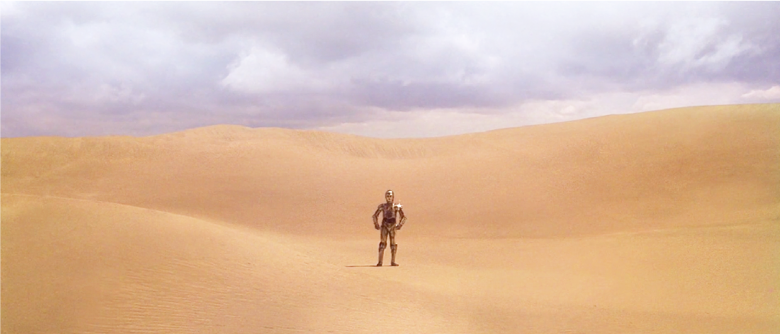
\includegraphics[width=\textwidth]{img/C3PONegativeSpace.png}
						\caption{Negative space.}
						\label{fig:NegativeSpace}
					\end{minipage}
				\end{figure}
				
				This technique also works in VR and is actually used in the intro of Henry.\todo{reference}.	By making everything but the subject equal or in a pattern, we can still grab peoples attention.\todo{improve or remove this}
				
				\todo{warning about how to use it}
				
				In figure \ref{fig:henryIntro} we can see how negative space is used in the intro of henry. They have a intro where you can sit down, some music starts playing and then slowly after the title card is displayed a story is told by a narrator and picture frames pop up to enhance the experience. this is an excellent use of negative space because it isn't used to focus your attention full time but rather to guide you to the starting point. People need a kind of pallet cleanser before going into such an experience. Just as you need to buy some popcorn, sit down and relax to see a movie before you can properly enjoy it. \todo{need to reference to a different chapter about how to start a vr experience} \todo{make sure to finish this}
				\begin{figure}[h]
					 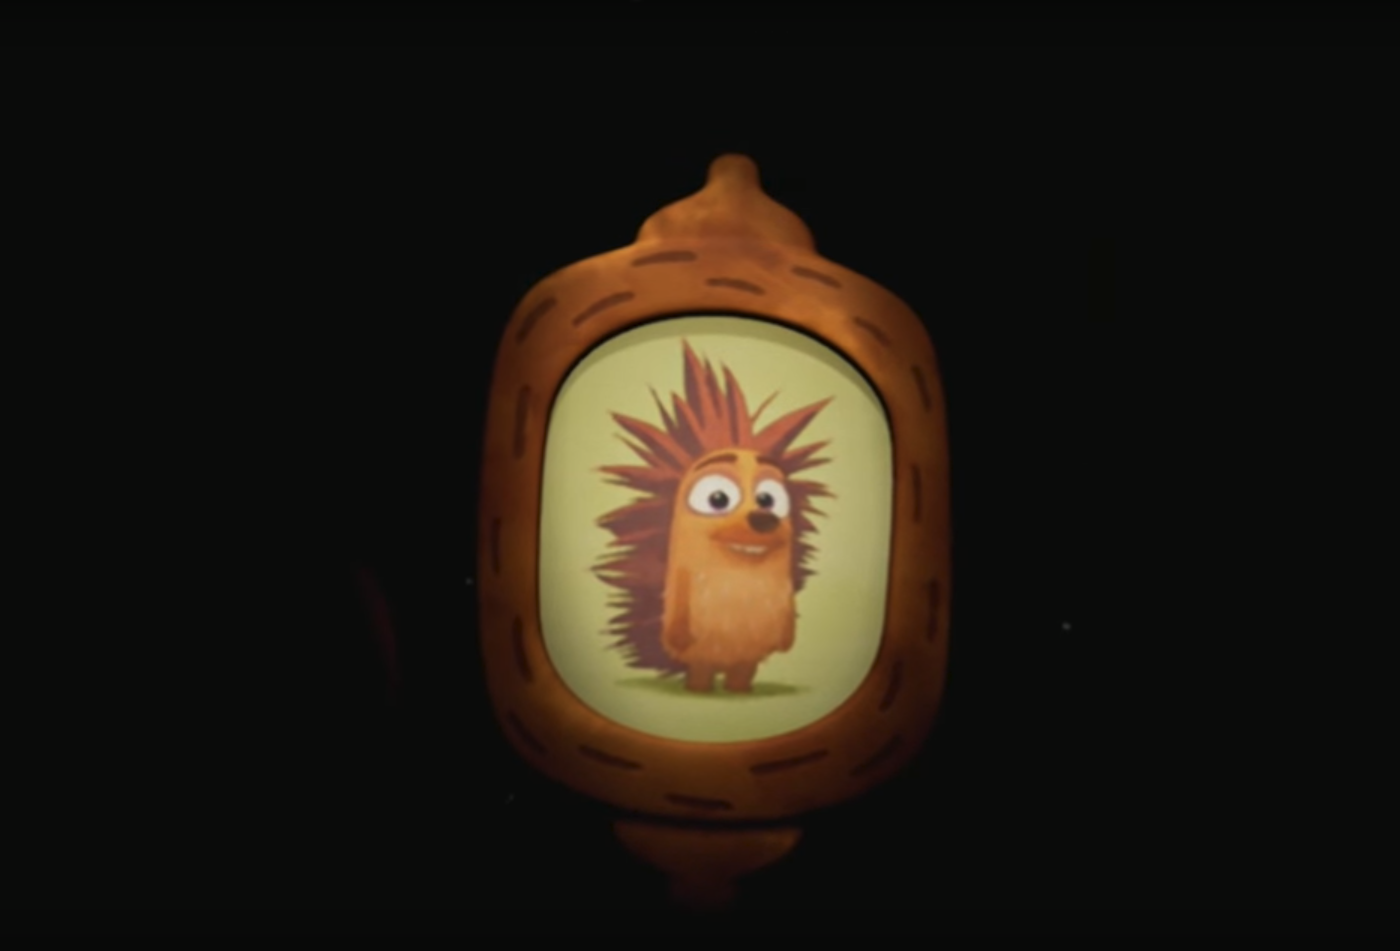
\includegraphics[width=\linewidth]{img/henry_intro.png}
					\caption{Intro of Henry.}
					\label{fig:henryIntro}
				\end{figure}
				\subsection{Guiding the attention} \todo{reread and adjust !!!!}
				
				Once you have the attention you have to keep it. This can be done by guiding the gaze. Dear angelica is an excellent example of this, it uses writing to grab and guide your attention. This way the user knows where to look but isn't limited to it. This is also one of the most important realisations to have as a director of a storytelling experience. Know that your audience might not be following your gaze!
				
				This means that you can try and try to have every moment of your environment be focused on your story, but still fail in achieving it in your viewers. Users can be quite different and might hang on to previous story points or may just simply be amazed by their surroundings. This is a key point of storytelling in VR.
				
				You can't completely focus all of you attention on one point. Now you might think, what if i make only one thing happen at a time. Surely the user will focus on the one thing that is interesting. Unfortunately this will make the world feel fake\todo{add citation of blog}. When only one thing around us is making noise or is interesting the entire world seems fake because the real world isn't like that. When people are put into sensory deprivation tanks the often begin to hallucinate because the brain needs input. Now of course people won't start hallucinating in VR because there still is a lot of input but if there is only one thing to focus on or happening at a particular time the world seems fake. 
				This has primarily to do with sound. Listen to what's around you right now and notice how there is sound coming from all directions. May it be the water running through the radiator, a clock gently ticking or cars driving by. Our brains filter out a lot of uninteresting noise, but when it isn't there the brain starts to notice.
				
				%phantom sound https://www.oculus.com/story-studio/blog/binaural-audio-for-narrative-vr/
				\subsection{Music and Narration}
								
				\chapter{Conclusion}
				\section{Where is VR storytelling currently}
				
				\section{Personal opinion}
				
				\section{The future of VR storytelling}
				
				\chapter{Sources}
				
				\section{Images}
				
				
				image pattern interrupt :\ref{fig:PatternInterrupt} \href{https://dealerwebb.com/WebSites/1626/Images/Blogs/2241/PatternInterrupt.jpg}{https://dealerwebb.com/WebSites/1626/Images/Blogs/2241/PatternInterrupt.jpg}
				
				star wars negative space :\ref{fig:NegativeSpace} \href{https://venngage-wordpress.s3.amazonaws.com/uploads/2015/12/negative-space.png}{https://venngage-wordpress.s3.amazonaws.com/uploads/2015/12/negative-space.png}
				
				Henry intro : \ref{fig:henryIntro} \href{https://youtu.be/IUY2yI5F16U}{https://youtu.be/IUY2yI5F16U}
				
				Pow attention image :\ref{fig:pow}
				\href{http://moziru.com/images/pop-art-clipart-pow-12.jpg}{http://moziru.com/images/pop-art-clipart-pow-12.jpg}
				
				\section{Literature}
				\bibliographystyle{apacite}
				\bibliography{bib.bib}
				
		\end{document}